\section{Introduction}
\label{sec:intro}

As robot sensing, perception and decision-making improves, the human's role in human-robot interaction progressively shifts from teleoperator to supervisor to teammate \cite{SchusterJentsch2013}.
This shift toward human-robot teaming means that the relationships between the human and the robot in a team to execute tasks together appear more and more to be collaboration.
Although there exists asymmetries between the capabilities and properties of a human and a robot, concepts from human-human teaming can be useful and important.
Specifically, the concept of a shared mental model, which originates from the theories of human collaboration, has been applied to analyze the collaborative process between humans and robots as well \cite{LebiereJentschOsosky2013}.

\begin{figure}[bph]
\centering
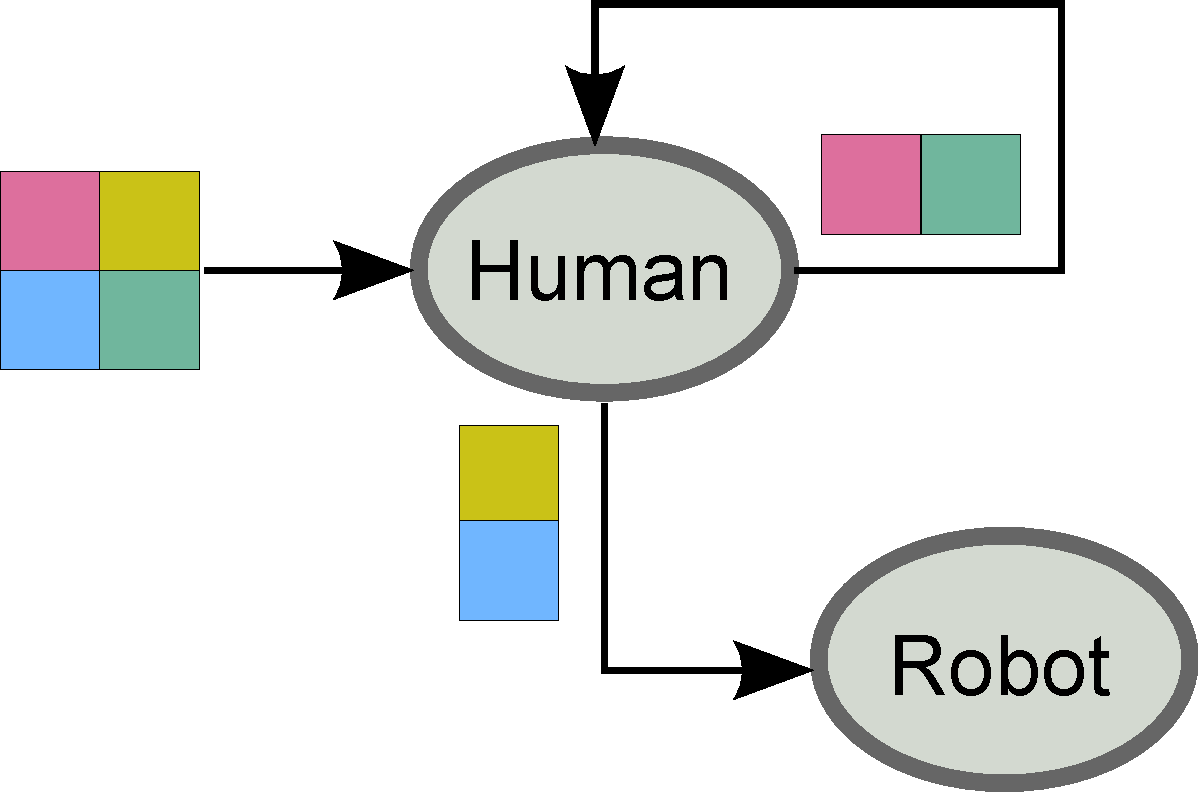
\includegraphics[width=0.35\linewidth]{./images/hrt}
\caption{An example of task-oriented human-robot collaboration.}
\label{fig:hrt}
\end{figure}

Consider a problem where team-wide collaboration is driven by a task shared by the team members.
The collaboration can be viewed as a parallel performance of the sub-tasks by different agents.
This type of collaboration can be modeled as a task decomposition.
In models created from a task decomposition, the team supervisor takes the responsibility of task decompositions and distributes the sub-tasks to different team members.
In a human-robot team, the team supervisor is usually a human.
%The collaboration between agents is usually driven by a task shared in the team.
%In order to maximize the team efficiency, the task is usually decomposed into several sub-tasks.
%The sub-tasks decrease the execution dependencies between agents in the team.
Figure \ref{fig:hrt} illustrates an example of task decomposition and allocation. 
%As a supervisor, the human usually determine how the task is decomposed and how to distribute to teammates.
A human supervisor decomposes the task into sub-tasks and then assign some to human team members and some to robot team members.

This type of relationship indicates the importance of the communication between a human and a robot.
Effective communication determines the execution efficiency and the correctness of the outcome.
One of the functions of the shared mental model is to facilitate the mutual understanding and ground communication among the team members.
%This model could be used to analyze the capabilities and the limitations of the team interaction so that the improvement could be proposed and applied.
%An effective communication between the human and the robot could greatly increase the team efficiency.
%The shared mental model is introduced to facilitate mutual understanding and ground communication.
%TODO: cite something here. 
Of particular importance is how shared mental models enable a more collaborative approach to problem solving, facilitated by communications that operate at a higher, more tactical or strategic level of abstraction.  
%In a collaborative level, people usually would like a complex process of parameter setup for a human to define a sub-task.
A complex process of parameter setup for a human to define a sub-task will reduce the team performance in a cordon and search task \cite{goodrich2013toward}.

In a cordon and search problem, a robot could be assigned to ``screen'' a sub-region that is not easily accessible to a human.
Instead of relying on teleoperation, the robot now can be autonomous enough to execute the sub-task alone.
In the collaborative perspective, the human only needs to express the requirements of the sub-task and provide information that the robot needs in sub-task execution.
In this paper, we assume that the team supervisor assigns the sub-tasks using a verbal command.
More specifically, we assume that the human supervisor issues directives to a robot.
Furthermore, we assume that from a small set of possible commands, the directives are grounded using spatial references that specify key locations for performing specific sub-tasks.
Finally, we assume that the directives are associated with a small number of adverbial modifiers that provide qualitative information about intent.
%If we do not expect that the team supervisor is an expert on robot parameter setup, the sub-task from the team supervisor is usually in a form of a verbal command.
%Often another expert is needed to translate the verbal command into parameter setup on the robot, which is an indirect human-robot interaction.
%It is obvious that a direct human-robot interaction can be a better way.

This does not require the robot to understand perfectly what the human said, but rather to model the verbal command.
%How to model the problem from human languages attracts plenty of research focuses.
The semantic elements in natural languages are often extracted and formed into a graphical model.
Bayesian inference can be applied to infer the meaning of a sentence \cite{conf/aaai/TellexKDWBTR11}. 
A learning process can also be imported to tune the likelihood of the primitives by using an HMM \cite{6343895}.
For tasks like cordon and search, plenty of the elements in a sentence depend on the spatial information in the workspace.
Thus, spatial labeling is imported to help convert a human's command into robot's navigation primitives \cite{5453186}.
This enables robot motion planning to be generated by a semantic interpreter \cite{6696345}.
In this paper, we are interested in modeling and solving a robot path-planning problem from a human's verbal command in a framework of task-oriented human-robot collaboration.

Current technologies can already support the language parsing process.
A semantic structure is usually composed of the key elements of a sentence, like a noun, verb and etc. 
Ignoring some other elements leads to information loss.
When researchers consider adverbial cues in human languages, an adverbial modifier may be modeled as belief revision \cite{Briggs:2011:FMM:2132890.2132916}.
We notice that a verbal command contains information not only what to do but also how to do.
It means that we should extract the search objectives and constraints from a verbal command to obtain the criteria.
The criteria evaluates the performance of a sub-task execution.

In this paper, we propose a framework to support the path-planning problem from a verbal command.
Using the idea of a shared mental model, we import a semantic labeling process to generate a semantic model of the workspace in Section \ref{sec:semantic}.
The labeled elements can be used to help the teammate interaction and task execution.
Specifically, we show how an optimization problem can be created by translating a verbal command.
We are interested in extracting information, like adverb elements, to create the multi-objective optimization in Section \ref{sec:moo}.
We propose an interactive method to find the optimal solution of a path-planning problem.
In Section \ref{sec:system}, we propose the system framework and the solutions on the robot path-planning.
